\documentclass[a4paper,12pt]{article}
\usepackage[utf8]{inputenc}
\usepackage[T1]{fontenc}
\usepackage[includeheadfoot,margin=2cm]{geometry}
\usepackage{times}
\usepackage{booktabs}
\usepackage[small,compact]{titlesec}
\usepackage{enumitem}
\usepackage{amsmath}
\usepackage{mathptmx}
\usepackage{tikz}
\usepackage{xifthen}
\frenchspacing
\setlist{nosep}
\renewcommand{\ttdefault}{cmtt}
\author{Thor Kristoffersen}
\date{\today}
\title{How to Build a Machine}
\newcommand{\num}[1]{\texttt{#1}}
\newcommand{\hex}[1]{\num{#1}_{\textup{\tiny 16}}}
\newcommand{\bin}[1]{\num{#1}_{\textup{\tiny 2}}}
\newcommand{\MEM}[1]{\ifthenelse{\equal{#1}{}}{M}{M[#1]}}
\newcommand{\PC}{P}
\newcommand{\SP}{S}
\newcommand{\TERM}{T}
\newcommand{\F}{\bin{0}}
\newcommand{\T}{\bin{1}}
\newcommand{\octno}[2]{#1.\mathrm{octet}[#2]}
\newcommand{\bitno}[2]{#1.\mathrm{bit}[#2]}
\newcommand{\range}[2]{\{#1,\ldots,#2\}}
\newcommand{\proc}[1]{\textsc{#1}}
\DeclareMathOperator{\MOD}{mod}
\newcommand{\modulo}[2]{#1 \MOD #2}
\newcommand{\comment}[1]{\begin{quote}[\textit{#1}]\end{quote}}
\newcommand{\op}[1]{$#1$}
\newcommand{\EXIT}      [1]{\op{\hex{00}}}
\newcommand{\NOP}       [1]{\op{\hex{01}}}
\newcommand{\JUMP}      [1]{\op{\hex{02}}}
\newcommand{\JUMPZERO}  [1]{\op{\hex{03}}}
\newcommand{\SETSP}     [1]{\op{\hex{04}}}
\newcommand{\GETPC}     [1]{\op{\hex{05}}}
\newcommand{\GETSP}     [1]{\op{\hex{06}}}
\newcommand{\PUSHZ}     [1]{\op{\hex{07}}}
\newcommand{\PUSHB}     [1]{\op{\hex{08}}}
\newcommand{\PUSHS}     [1]{\op{\hex{09}}}
\newcommand{\PUSHI}     [1]{\op{\hex{0A}}}
\newcommand{\PUSHL}     [1]{\op{\hex{0B}}}
\newcommand{\SIGXB}     [1]{\op{\hex{0C}}}
\newcommand{\SIGXS}     [1]{\op{\hex{0D}}}
\newcommand{\SIGXI}     [1]{\op{\hex{0E}}}
\newcommand{\LOADB}     [1]{\op{\hex{10}}}
\newcommand{\LOADS}     [1]{\op{\hex{11}}}
\newcommand{\LOADI}     [1]{\op{\hex{12}}}
\newcommand{\LOADL}     [1]{\op{\hex{13}}}
\newcommand{\STOREB}    [1]{\op{\hex{14}}}
\newcommand{\STORES}    [1]{\op{\hex{15}}}
\newcommand{\STOREI}    [1]{\op{\hex{16}}}
\newcommand{\STOREL}    [1]{\op{\hex{17}}}
\newcommand{\ADD}       [1]{\op{\hex{20}}}
\newcommand{\MULT}      [1]{\op{\hex{21}}}
\newcommand{\DIV}       [1]{\op{\hex{22}}}
\newcommand{\REM}       [1]{\op{\hex{23}}}
\newcommand{\LT}        [1]{\op{\hex{24}}}
\newcommand{\AND}       [1]{\op{\hex{28}}}
\newcommand{\OR}        [1]{\op{\hex{29}}}
\newcommand{\NOT}       [1]{\op{\hex{2A}}}
\newcommand{\XOR}       [1]{\op{\hex{2B}}}
\newcommand{\POW}       [1]{\op{\hex{2C}}}
\newcommand{\NEWFRAME}  [1]{\op{\hex{30}}}
\newcommand{\SETPIXEL}  [1]{\op{\hex{31}}}
\newcommand{\ADDSAMPLE} [1]{\op{\hex{32}}}
\newcommand{\PUTCHAR}   [1]{\op{\hex{34}}}
\newcommand{\READFRAME} [1]{\op{\hex{38}}}
\newcommand{\READPIXEL} [1]{\op{\hex{39}}}

\newlist{stepnumbers}{enumerate}{2}
\setlist[stepnumbers]{label=\arabic*.}
\newlist{stepletters}{enumerate}{1}
\setlist[stepletters]{label=\alph*.}

\begin{document}

\maketitle

\noindent
This film contains programs that can be executed by a machine.
The purpose of this part of the film is to guide you through the process of building this machine.
Using this guide, it should be possible for one person to build a machine in a week.
To understand the guide, it is necessary to have knowledge of basic 20th-century mathematics and physics.

When you have finished the machine, you will need to install an initial program in it before you can use it to execute programs.
This initial program is supplied as part of the film.

You will start by building a very simple machine, and then you will extend this machine through several stages, so that by the end you will have a fully functional machine.
Only when you have obtained the correct test results for each stage should you proceed with the following stage.

Number systems used here include decimal, binary, and hexadecimal.
All non-decimal numbers are explictly indicated by subscripts indicating the number base in decimal.
Further detail on binary and hexadecimal notation can be found in Appendix~\ref{sec:number-notation}.

\section{Storage}

To build the machine, you first need some form of storage to represent state consisting of binary digits (bits).

\subsection{Representing State}

An \emph{element} is a group of bits in the storage that forms a unit with respect to naming.
The number of bits in an element is called the \emph{size} of the element.
Each element has a unique name, so that it can be unambiguously referred to, and the contents can be retrieved or stored in one atomic operation.
The following elements are employed by the machine:
\begin{description}
\item[1-bit elements]
  $\TERM$ is a one 1-bit element.
\item[8-bit elements]
  $\MEM{}$ is an array of $2^N$ 8-bit elements that is indexed by an integer in the range from $0$ to $2^N - 1$, for $N \le 64$.
  The element at index $i$ in $\MEM{}$ is named $\MEM{i}$.
  $N$ is a constant that must be known at the time the machine is started.
\item[64-bit elements]
  $\PC$ and $\SP$ are 64-bit elements.
\end{description}
In addition to the elements defined in this list, it will be necessary for some tasks to use some temporary elements.
This is explained in Section~\ref{sec:storage-operations}

\subsection{Notation}

For any element, $x$, the notation $\bitno{x}{i}$ refers to bit $i$ in $x$.

A group of 8 bits is called an \emph{octet}, and in a 64-bit element, $x$, the notation $\octno{x}{i}$ refers to octet $i$ in $x$, which is the octet consisting of the bits from $\bitno{x}{8i+7}$ to $\bitno{x}{8i}$.

The modulo operation, $\modulo{x}{y}$, for $y>0$, is defined here as follows:
\[ \modulo{x}{y} = x - y \left \lfloor \frac{x}{y} \right \rfloor \]
where $\left \lfloor x \right \rfloor$ is defined as the unique integer such that $\left \lfloor x \right \rfloor \le x < (\left \lfloor x \right \rfloor + 1)$.
    
\subsection{Operations}
\label{sec:storage-operations}

We need to define a few terms to talk about storage.
These should be basic operations in your implementation.
\begin{itemize}
\item ``The value of an element.'' means the contents as retrieved from that element.
\item ``To set an element to $x$'' means to store the value of $x$ in that element.
\item ``The value of an octet.'' means the contents as retrieved from that octet.
\item ``To set an octet to $x$'' means to store the value of $x$ in that octet, while keeping all other contents unchanged.
\item ``To increment an element by $n$'' means to set $x$ to the value of the element and then set that element to $\modulo{(x + n)}{2^s}$, where $s$ is the size of the element.
\item ``To decrement an element by $n$'' means to set $x$ to the value of the element and then set that element to $\modulo{(x - n)}{2^s}$, where $s$ is the size of the element.
\item  ``To initialize the temporary $n$-bit element $x$ to $k$'' means to create a temporary element of size $n$, name it $x$, and store the value of $k$ in $x$.
\end{itemize}

\subsection{Testing the Storage Operations}

To test that the storage works as it should, do the following tests many times for $\PC$, $\SP$, $\TERM$, and $\MEM{i}$, where $i \in \range{0}{2^N-1}$ and $N=8$.

\subsubsection{Element Values}

Verify that your operations for storing and getting the value of an element work for every element, $x$, of size $s$.
\begin{stepnumbers}
\item Initialize the temporary element, $y$, of size $s$.
\item For all $i \in \range{0}{s-1}$, set $\bitno{y}{i}$ to a random bit value.
\item Set $x$ to $y$.
\item Verify that $x = y$.
\end{stepnumbers}

\subsubsection{Incrementing and Decrementing}

Verify that your operations for incrementing and decrementing an element work for every element, $x$, of size $s$.
\begin{stepnumbers}
\item Initialize the temporary elements, $y$ and $z$, of size $s$.
\item For all $i \in \range{0}{s-1}$, set $\bitno{y}{i}$ to a random bit value.
\item For all $i \in \range{0}{s-1}$, set $\bitno{z}{i}$ to a random bit value.
\item Set $x$ to $y$.
\item Increment $x$ by $z$.
\item Verify that $x = \modulo{(y + z)}{2^s}$.
\item Decrement $x$ by $z$.
\item Verify that $x = y$.
\end{stepnumbers}

\subsubsection{Octets}

Verify that your octet operations work for every 64-bit element, $x$, and every octet, $\octno{x}{n}$ where $n \in \range{0}{7}$.
\begin{stepnumbers}
\item Initialize the temporary element, $y$, of size 64.
\item Initialize the temporary element, $z$, of size 8.
\item For all $i \in \range{0}{s-1}$, set $\bitno{y}{i}$ to a random bit value.
\item For all $i \in \range{0}{7}$, set $\bitno{z}{i}$ to a random bit value.
\item Set $x$ to $y$.
\item Set $\octno{x}{n}$ to $z$.
\item Verify that $\octno{x}{n} = z$.
\item Verify that $\octno{x}{i} = \octno{y}{i}$ where $i \in \range{0}{7}$ and $i \neq n$.
\end{stepnumbers}


\section{Basic Procedures}

You will need to implement six basic procedures that are frequently used by the machine.
These use the storage operations described in Section~\ref{sec:storage-operations}.

\subsection{Descriptions of Procedures}

\subsubsection{\proc{Put} Octets}

Assume that we have two temporary 64-bit elements called $x$ and $a$, and that $n$ is either 1, 2, 4, or 8.
The expression ``\proc{Put} $n$ octets from $x$ into index $a$'' means to do the following steps:
\begin{stepnumbers}
\item Initialize the temporary 8-bit element $i$ to 0.
\item Do the following $n$ times:
  \begin{stepletters}
  \item Set $\MEM{a+i}$ to $\octno{x}{i}$.
  \item Increment $i$ by 1.
  \end{stepletters}
\end{stepnumbers}

\subsubsection{\proc{Get} Octets}

Assume that we have a temporary 64-bit element called $a$ and that $n$ is either 1, 2, 4, or 8.
The expression ``\proc{Get} $n$ octets from index $a$ into $x$'' means to do the following steps:
\begin{stepnumbers}
\item Initialize the temporary 64-bit element $x$ to 0.
\item Initialize the temporary 8-bit element $i$ to 0.
\item Do the following $n$ times:
  \begin{stepletters}
  \item Set $\octno{x}{i}$ to $\MEM{a+i}$.
  \item Increment $i$ by 1.
  \end{stepletters}
\end{stepnumbers}
The temporary 64-bit element $x$ can now be used by other procedures.

\subsubsection{\proc{Push} Element}

Assume that we have a temporary 64-bit element called $x$.
The expression ``\proc{Push} $x$'' means to do the following steps:
\begin{stepnumbers}
\item Decrement $\SP$ by 8.
\item \proc{Put} 8 octets from $x$ into index $\SP$.
\end{stepnumbers}

\subsubsection{\proc{Pop} Element}

The expression ``\proc{Pop} $x$'' means to do the following steps:
\begin{stepnumbers}
\item Initialize the temporary 64-bit element $x$ to 0.
\item \proc{Get} 8 octets from index $\SP$ into $x$.
\item Increment $\SP$ by 8.
\end{stepnumbers}
The 64-bit element $x$ can now be used by other procedures.

\subsubsection{\proc{Fetch} Octets}

Assume that $n$ is either 1, 2, 4, or 8.
The expression ``\proc{Fetch} $n$ octets into $x$'' means to do the following steps:
\begin{stepnumbers}
\item Initialize the temporary 64-bit element $x$ to 0.
\item \proc{Get} $n$ octets from index $\PC$ into $x$.
\item Increment $\PC$ by $n$.
\end{stepnumbers}
The temporary 64-bit element $x$ can now be used by other procedures.

\subsubsection{\proc{Extend} Sign}

Assume that we have a temporary 64-bit element called $x$ and that $n$ is either 1, 2, or 4.
The expression ``\proc{Extend} sign for $n$ octets in $x$'' means to do the following step:
\begin{stepnumbers}
\item If the value of $\bitno{x}{8n-1}$ is 1, then for all $i \in \range{8n}{63}$ set $\bitno{x}{i}$ to 1.
\end{stepnumbers}
The temporary 64-bit element $x$ can now be used by other procedures.

\subsection{Testing the Basic Procedures}

\subsubsection{Testing \proc{Put} and \proc{Get}}

To test \proc{Put} and \proc{Get}, do as follows, with $N=4$:
\begin{stepnumbers}
\item Set $M[i]$ to 0 for all $i \in \range{0}{2^N-1}$.
\item Initialize the temporary 64-bit element $x$ to $\hex{0123456789ABCDEF}$.
\item \proc{Put} 1 octet  from $x$ into index $\hex{01}$.
\item \proc{Put} 2 octets from $x$ into index $\hex{02}$.
\item \proc{Put} 4 octets from $x$ into index $\hex{04}$.
\item \proc{Put} 8 octets from $x$ into index $\hex{08}$.
\item \proc{Get} 1 octet  from index $\hex{0E}$ into $x$ .
\item Verify that the value of $x$ is $\hex{0000000000000023}$.
\item \proc{Get} 2 octets from index $\hex{0C}$ into $x$ .
\item Verify that the value of $x$ is $\hex{0000000000004567}$.
\item \proc{Get} 4 octets from index $\hex{08}$ into $x$ .
\item Verify that the value of $x$ is $\hex{0000000089ABCDEF}$.
\item \proc{Get} 8 octets from index $\hex{00}$ into $x$ .
\item Verify that the value of $x$ is $\hex{89ABCDEFCDEFEF00}$.
\item Verify that the contents of the elements in $\MEM{}$ are as in the following table.
\end{stepnumbers}

\begin{center}
  \begin{tabular}{@{}lr@{}}
    \hline
    Element        & Value    \\
    \hline
    $\hex{0000000000000000}$ & $\hex{00}$ \\
    $\hex{0000000000000001}$ & $\hex{EF}$ \\
    $\hex{0000000000000002}$ & $\hex{EF}$ \\
    $\hex{0000000000000003}$ & $\hex{CD}$ \\
    $\hex{0000000000000004}$ & $\hex{EF}$ \\
    $\hex{0000000000000005}$ & $\hex{CD}$ \\
    $\hex{0000000000000006}$ & $\hex{AB}$ \\
    $\hex{0000000000000007}$ & $\hex{89}$ \\
    \hline
  \end{tabular}
  \hfil
  \begin{tabular}{@{}lr@{}}
    \hline
    Element        & Value    \\
    \hline
    $\hex{0000000000000008}$ & $\hex{EF}$ \\
    $\hex{0000000000000009}$ & $\hex{CD}$ \\
    $\hex{000000000000000A}$ & $\hex{AB}$ \\
    $\hex{000000000000000B}$ & $\hex{89}$ \\
    $\hex{000000000000000C}$ & $\hex{67}$ \\
    $\hex{000000000000000D}$ & $\hex{45}$ \\
    $\hex{000000000000000E}$ & $\hex{23}$ \\
    $\hex{000000000000000F}$ & $\hex{01}$ \\
    \hline
  \end{tabular}
\end{center}

\subsubsection{Testing \proc{Push} and \proc{Pop}}

To test \proc{Push} and \proc{Pop}, do as follows, with $N=3$:
\begin{stepnumbers}
\item Set $M[i]$ to 0 for all $i \in \range{0}{2^N-1}$.
\item Set $\SP$ to $\hex{08}$.
\item Initialize the temporary 64-bit element $x$ to $\hex{0123456789ABCDEF}$.
\item Initialize the temporary 64-bit element $y$ to $0$.
\item \proc{Push} $x$.
\item Verify that the value of $\SP$ is $\hex{00}$.
\item \proc{Pop} $y$.
\item Verify that $x=y$.
\item Verify that the value of $\SP$ is $\hex{08}$.
\end{stepnumbers}

\subsubsection{Testing \proc{Fetch} and \proc{Extend}}

To test \proc{Fetch} and \proc{Extend}, do as follows, with $N=4$:
\begin{stepnumbers}
\item Set $M[i]$ to 0 for all $i \in \range{0}{2^N-1}$.
\item Initialize the temporary 64-bit element $w$ to 0.
\item Initialize the temporary 64-bit element $x$ to $\hex{0000000000000080}$.
\item \proc{Extend} sign for 1 octet in $x$.
\item Verify that the value of $x$ is $\hex{FFFFFFFFFFFFFF80}$.
\item \proc{Put} 8 octets from $x$ into index 0.
\item \proc{Fetch} 1 octet into $w$.
\item Verify that the value of $w$ is $\hex{0000000000000080}$.
\item Verify that the value of $\PC$ is 1.
\item Initialize the temporary 64-bit element $y$ to $\hex{0000000000008000}$.
\item \proc{Extend} sign for 2 octets in $y$.
\item Verify that the value of $y$ is $\hex{FFFFFFFFFFFF8000}$.
\item \proc{Put} 8 octets from $y$ into index 0.
\item \proc{Fetch} 2 octets into $w$.
\item Verify that the value of $w$ is $\hex{000000000000FF80}$.
\item Verify that the value of $\PC$ is 3.
\item Initialize the temporary 64-bit element $z$ to $\hex{0000000080000000}$.
\item \proc{Extend} sign for 4 octets in $z$.
\item Verify that the value of $z$ is $\hex{FFFFFFFF80000000}$.
\item \proc{Put} 8 octets from $z$ into index 0.
\item \proc{Fetch} 4 octets into $w$.
\item Verify that the value of $w$ is $\hex{00000000FFFFFF80}$.
\item Verify that the value of $\PC$ is 7.
\item \proc{Fetch} 8 octets into $w$.
\item Verify that the value of $w$ is $\hex{00000000000000FF}$.
\item Verify that the value of $\PC$ is 15.
\end{stepnumbers}

\section{First Version of The Machine}

You can now proceed with implementing a basic version of the machine with $N=8$.

Machine operation proceeds through two phases: first the storage is set up, and then the main procedure is executed.

\subsection{Setting Up the Storage}

To set up the storage, you need to set all elements to predefined values.
$\MEM{i}$ is set to 0 for every $i \in \range{0}{2^N-1}$, $\PC$ is set to $0$, and $\SP$ is set to $2^N$.
The values are given in the table below.

\begin{center}
  \begin{tabular}{@{}lr@{}}
    \hline
    Element  & Value                   \\
    \hline
    $\TERM$          & $\F$                      \\
    $\PC$            & $\hex{0000000000000000}$  \\
    $\SP$            & $\hex{0000000000000100}$  \\
    \hline
  \end{tabular}
\end{center}

\subsection{The Main Procedure}

When you have set up the storage, execute the main procedure repeatedly until the value of $\TERM$ is $\T$.
The main procedure must carry out the following steps.
\begin{stepnumbers}
\item Initialize the temporary 64-bit element $k$ to 0.
\item \proc{Fetch} 1 octet into $k$.
\item\label{itm:main-case} If the value of $k$ is
  \begin{description}
  \item[\NOP{}] then do nothing.
  \item[\JUMP{}] then
    \begin{stepnumbers}
    \item Initialize the temporary 64-bit element $a$ to 0.
    \item \proc{Pop} $a$.
    \item Set $\PC$ to $a$.
    \end{stepnumbers}
  \item[\JUMPZERO{}] then
    \begin{stepnumbers}
    \item Initialize the temporary 64-bit elements $a$ and $x$ to 0.
    \item \proc{Fetch} 1 octet into $a$.
    \item \proc{Extend} sign for 1 octet in $a$.
    \item \proc{Pop} $x$.
    \item If the value of $x$ is 0, then increment $\PC$ by $a$.
    \end{stepnumbers}
  \item[\SETSP{}] then
    \begin{stepnumbers}
    \item Initialize the temporary 64-bit element $a$ to 0.
    \item \proc{Pop} $a$.
    \item Set $\SP$ to $a$.
    \end{stepnumbers}
  \item[\GETPC{}] then
    \begin{stepnumbers}
    \item Initialize the temporary 64-bit element $a$ to $\PC$.
    \item \proc{Push} $a$.
    \end{stepnumbers}
  \item[\GETSP{}] then
    \begin{stepnumbers}
    \item Initialize the temporary 64-bit element $a$ to $\SP$.
    \item \proc{Push} $a$.
    \end{stepnumbers}
  \item[\PUSHL{}] then
    \begin{stepnumbers}
    \item Initialize the temporary 64-bit element $a$ to 0.
    \item \proc{Fetch} 8 octets into $a$.
    \item \proc{Push} $a$.
    \end{stepnumbers}
  \end{description}
\item If the value of $k$ does not occur in the list in the previous point, then set $\TERM$ to $\T$.
\end{stepnumbers}

\subsection{Testing the Basic Machine}

To test the machine, set the following elements to the provided values.

\begin{center}
  \begin{tabular}{@{}ll@{}}
    \hline
    Element    & Value \\
    \hline
    $\hex{00}$ & $\hex{01}$ \\
    $\hex{01}$ & $\hex{0B}$ \\
    $\hex{02}$ & $\hex{23}$ \\
    $\hex{03}$ & $\hex{00}$ \\
    $\hex{04}$ & $\hex{00}$ \\
    $\hex{05}$ & $\hex{00}$ \\
    $\hex{06}$ & $\hex{00}$ \\
    $\hex{07}$ & $\hex{00}$ \\
    $\hex{08}$ & $\hex{00}$ \\
    $\hex{09}$ & $\hex{00}$ \\
    $\hex{0A}$ & $\hex{0B}$ \\
    $\hex{0B}$ & $\hex{01}$ \\
    $\hex{0C}$ & $\hex{00}$ \\
    $\hex{0D}$ & $\hex{00}$ \\
    $\hex{0E}$ & $\hex{00}$ \\
    $\hex{0F}$ & $\hex{00}$ \\
    \hline
  \end{tabular}
  \hfil
  \begin{tabular}{@{}ll@{}}
    \hline
    Element    & Value \\
    \hline
    $\hex{10}$ & $\hex{00}$ \\
    $\hex{11}$ & $\hex{00}$ \\
    $\hex{12}$ & $\hex{00}$ \\
    $\hex{13}$ & $\hex{0B}$ \\
    $\hex{14}$ & $\hex{00}$ \\
    $\hex{15}$ & $\hex{00}$ \\
    $\hex{16}$ & $\hex{00}$ \\
    $\hex{17}$ & $\hex{00}$ \\
    $\hex{18}$ & $\hex{00}$ \\
    $\hex{19}$ & $\hex{00}$ \\
    $\hex{1A}$ & $\hex{00}$ \\
    $\hex{1B}$ & $\hex{00}$ \\
    $\hex{1C}$ & $\hex{03}$ \\
    $\hex{1D}$ & $\hex{01}$ \\
    $\hex{1E}$ & $\hex{00}$ \\
    $\hex{1F}$ & $\hex{03}$ \\
    \hline
  \end{tabular}
  \hfil
  \begin{tabular}{@{}ll@{}}
    \hline
    Element    & Value \\
    \hline
    $\hex{20}$ & $\hex{01}$ \\
    $\hex{21}$ & $\hex{02}$ \\
    $\hex{22}$ & $\hex{00}$ \\
    $\hex{23}$ & $\hex{06}$ \\
    $\hex{24}$ & $\hex{05}$ \\
    $\hex{25}$ & $\hex{0B}$ \\
    $\hex{26}$ & $\hex{F8}$ \\
    $\hex{27}$ & $\hex{00}$ \\
    $\hex{28}$ & $\hex{00}$ \\
    $\hex{29}$ & $\hex{00}$ \\
    $\hex{2A}$ & $\hex{00}$ \\
    $\hex{2B}$ & $\hex{00}$ \\
    $\hex{2C}$ & $\hex{00}$ \\
    $\hex{2D}$ & $\hex{00}$ \\
    $\hex{2E}$ & $\hex{04}$ \\
    $\hex{2F}$ & $\hex{00}$ \\
    \hline
  \end{tabular}
\end{center}

Now start the machine.
When it terminates, all elements should remain unchanged, except the following ones, which should have the indicated values, otherwise the implementation is incorrect.

\begin{center}
  \begin{tabular}{@{}lr@{}}
    \hline
    Element          & Value                     \\
    \hline
    $\TERM$          & $\T$                      \\
    $\PC$            & $\hex{0000000000000030}$ \\
    $\SP$            & $\hex{00000000000000F8}$ \\
    $\MEM{\hex{E8}}$ & $\hex{F8}$ \\
    $\MEM{\hex{F0}}$ & $\hex{25}$ \\
    $\MEM{\hex{F9}}$ & $\hex{01}$ \\
    \hline
  \end{tabular}
\end{center}

\section{Second Version of the Machine}

In the next version of the machine you will add several more cases to step \ref{itm:main-case} of the main procedure.

\begin{stepnumbers}[start=3]
\item If $k$ is
  \begin{description}
  \item[\LOADL{}] then
    \begin{stepnumbers}
    \item Initialize the temporary 64-bit elements $a$ and $x$ to 0.
    \item \proc{Pop} $a$.
    \item \proc{Get} 8 octets from index $a$ into $x$.
    \item \proc{Push} $x$.
    \end{stepnumbers}
  \item[\STOREL{}] then
    \begin{stepnumbers}
    \item Initialize the temporary 64-bit elements $a$ and $x$ to 0.
    \item \proc{Pop} $a$.
    \item \proc{Pop} $x$.
    \item \proc{Put} 8 octets from $x$ into index $a$.
    \end{stepnumbers}
  \item[\ADD{}] then
    \begin{stepnumbers}
    \item Initialize the temporary 64-bit elements $x$ and $y$ to 0.
    \item \proc{Pop} $y$.
    \item \proc{Pop} $x$.
    \item \proc{Push} $\modulo{(x + y)}{2^{64}}$.
    \end{stepnumbers}
  \item[\MULT{}] then
    \begin{stepnumbers}
    \item Initialize the temporary 64-bit elements $x$ and $y$ to 0.
    \item \proc{Pop} $y$.
    \item \proc{Pop} $x$.
    \item \proc{Push} $\modulo{(x y)}{2^{64}}$.
    \end{stepnumbers}
  \item[\DIV{}] then
    \begin{stepnumbers}
    \item Initialize the temporary 64-bit elements $x$ and $y$ to 0.
    \item \proc{Pop} $y$.
    \item \proc{Pop} $x$.
    \item If $x > 0$ and $y > 0$,
      \begin{itemize}[label=]
      \item then \proc{Push} $q$, such that $x = qy + r$ and $0 \leq r < y$,
      \item otherwise \proc{Push} 0.
      \end{itemize}
    \end{stepnumbers}
  \item[\REM{}] then
    \begin{stepnumbers}
    \item Initialize the temporary 64-bit elements $x$ and $y$ to 0.
    \item \proc{Pop} $y$.
    \item \proc{Pop} $x$.
    \item If $x > 0$ and $y > 0$,
      \begin{itemize}[label=]
      \item then \proc{Push} $r$, such that $x = qy + r$ and $0 \leq r < y$,
      \item otherwise \proc{Push} 0.
      \end{itemize}
    \end{stepnumbers}
  \item[\LT{}] then
    \begin{stepnumbers}
    \item Initialize the temporary 64-bit elements $x$ and $y$ to 0.
    \item \proc{Pop} $y$.
    \item \proc{Pop} $x$.
    \item If $x < y$,
      \begin{itemize}[label=]
      \item then \proc{Push} $2^{64} - 1$,
      \item otherwise \proc{Push} 0.
      \end{itemize}
    \end{stepnumbers}
  \item[\AND{}] then
    \begin{stepnumbers}
    \item Initialize the temporary 64-bit elements $x$, $y$, and $z$ to 0.
    \item \proc{Pop} $y$.
    \item \proc{Pop} $x$.
    \item For every $i \in \range{0}{63}$, if $\bitno{x}{i}$ is 1 and $\bitno{y}{i}$ is 1,
      \begin{itemize}[label=]
      \item then set $\bitno{z}{i}$ to 1,
      \item otherwise set $\bitno{z}{i}$ 0.
      \end{itemize}
    \item \proc{Push} $z$.
    \end{stepnumbers}
  \item[\OR{}] then
    \begin{stepnumbers}
    \item Initialize the temporary 64-bit elements $x$, $y$, and $z$ to 0.
    \item \proc{Pop} $y$.
    \item \proc{Pop} $x$.
    \item For every $i \in \range{0}{63}$, if $\bitno{x}{i}$ is 0 and $\bitno{y}{i}$ is 0,
      \begin{itemize}[label=]
      \item then set $\bitno{z}{i}$ to 0,
      \item otherwise set $\bitno{z}{i}$ to 1.
      \end{itemize}
    \item \proc{Push} $z$.
    \end{stepnumbers}
  \item[\NOT{}] then
    \begin{stepnumbers}
    \item Initialize the temporary 64-bit elements $x$ and $z$ to 0.
    \item \proc{Pop} $x$.
    \item For every $i \in \range{0}{63}$, if $\bitno{x}{i}$ is 1,
      \begin{itemize}[label=]
      \item then set $\bitno{z}{i}$ to 0,
      \item otherwise set $\bitno{z}{i}$ to 1.
      \end{itemize}
    \item \proc{Push} $z$.
    \end{stepnumbers}
  \item[\XOR{}] then
    \begin{stepnumbers}
    \item Initialize the temporary 64-bit elements $x$, $y$, and $z$ to 0.
    \item \proc{Pop} $y$.
    \item \proc{Pop} $x$.
    \item For every $i \in \range{0}{63}$, if $\bitno{x}{i}$ is different from $\bitno{y}{i}$,
      \begin{itemize}[label=]
      \item then set $\bitno{z}{i}$ to 1,
      \item otherwise set $\bitno{z}{i}$ to 0.
      \end{itemize}
    \item \proc{Push} the 64-bit value $z$.
    \end{stepnumbers}
  \item[\POW{}] then
    \begin{stepnumbers}
    \item Initialize the temporary 64-bit element $x$ to 0.
    \item \proc{Pop} $x$.
    \item If $x < 64$,
      \begin{itemize}[label=]
      \item then \proc{Push} $2^x$,
      \item otherwise \proc{Push} 0.
      \end{itemize}
    \end{stepnumbers}
  \end{description}
\end{stepnumbers}

\comment{More tests here.}

\section{Third Version of the Machine}

In the third version of the machine you will add still more cases to step \ref{itm:main-case} of the main procedure.

\begin{stepnumbers}[start=3]
\item If $k$ is
  \begin{description}
  \item[\PUSHB{}] then
    \begin{stepnumbers}
    \item Initialize the temporary 64-bit element $a$ to 0.
    \item \proc{Fetch} 1 octet into $a$.
    \item \proc{Push} $a$.
    \end{stepnumbers}
  \item[\PUSHS{}] then
    \begin{stepnumbers}
    \item Initialize the temporary 64-bit element $a$ to 0.
    \item \proc{Fetch} 2 octets into $a$.
    \item \proc{Push} $a$.
    \end{stepnumbers}
  \item[\PUSHI{}] then
    \begin{stepnumbers}
    \item Initialize the temporary 64-bit element $a$ to 0.
    \item \proc{Fetch} 4 octets into $a$.
    \item \proc{Push} $a$.
    \end{stepnumbers}
  \item[\SIGXB{}] then
    \begin{stepnumbers}
    \item Initialize the temporary 64-bit element $x$ to 0.
    \item \proc{Pop} $x$.
    \item \proc{Extend} sign for 1 octet in $x$.
    \item \proc{Push} $x$.
    \end{stepnumbers}
  \item[\SIGXS{}] then
    \begin{stepnumbers}
    \item Initialize the temporary 64-bit element $x$ to 0.
    \item \proc{Pop} $x$.
    \item \proc{Extend} sign for 2 octets in $x$.
    \item \proc{Push} $x$.
    \end{stepnumbers}
  \item[\SIGXI{}] then
    \begin{stepnumbers}
    \item Initialize the temporary 64-bit element $x$ to 0.
    \item \proc{Pop} $x$.
    \item \proc{Extend} sign for 4 octets in $x$.
    \item \proc{Push} $x$.
    \end{stepnumbers}
  \item[\LOADB{}] then
    \begin{stepnumbers}
    \item Initialize the temporary 64-bit element $a$ to 0.
    \item \proc{Pop} $a$.
    \item \proc{Get} 1 octet from index $a$ into $x$.
    \item \proc{Push} $x$.
    \end{stepnumbers}
  \item[\LOADS{}] then
    \begin{stepnumbers}
    \item Initialize the temporary 64-bit element $a$ to 0.
    \item \proc{Pop} $a$.
    \item \proc{Get} 2 octets from index $a$ into $x$.
    \item \proc{Push} $x$.
    \end{stepnumbers}
  \item[\LOADI{}] then
    \begin{stepnumbers}
    \item Initialize the temporary 64-bit element $a$ to 0.
    \item \proc{Pop} $a$.
    \item \proc{Get} 4 octets from index $a$ into $x$.
    \item \proc{Push} $x$.
    \end{stepnumbers}
  \item[\STOREB{}] then
    \begin{stepnumbers}
    \item Initialize the temporary 64-bit elements $a$ and $x$ to 0.
    \item \proc{Pop} $a$.
    \item \proc{Pop} $x$.
    \item \proc{Put} 1 octet from $x$ into index $a$.
    \end{stepnumbers}
  \item[\STORES{}] then
    \begin{stepnumbers}
    \item Initialize the temporary 64-bit elements $a$ and $x$ to 0.
    \item \proc{Pop} $a$.
    \item \proc{Pop} $x$.
    \item \proc{Put} 2 octets from $x$ into index $a$.
    \end{stepnumbers}
  \item[\STOREI{}] then
    \begin{stepnumbers}
    \item Initialize the temporary 64-bit elements $a$ and $x$ to 0.
    \item \proc{Pop} $a$.
    \item \proc{Pop} $x$.
    \item \proc{Put} 4 octets from $x$ into index $a$.
    \end{stepnumbers}
  \end{description}
\end{stepnumbers}

\comment{More tests here.}

\section{Building the Devices}
\label{sec:building-devices}

At this point you should have a machine with fully functional computational capabilities.
What's missing are the devices that allow the machine to consume data from its environment and to produce data to its environment.
There are four devices:
\begin{itemize}
\item The \emph{Image Input} device allows the machine to consume images as a two-dimensional array of gray-scale values.
  This device is very important, because it is what enables the machine to load programs encoded as images on the film.
\item The \emph{Image Output} device allows the machine to produce color images.
  Moving images are supported by producing a time series of still images.
\item The \emph{Audio Output} device allows the machine to produce audio signals as a time series of amplitude values.
\item The \emph{Text Output} device allows the machine to produce text as a stream of characters.
\end{itemize}
The descriptions below will only explain the correspondence between machine events and real world events.
It is up to you to make sure that the interpretation of real world events is faithfully implemented.

\subsection{Image Input}

The \emph{Image Input} device allows the machine to consume an image as a two-dimensional array of points of light intensity values.
The following figure shows an example of such an array, consisting of 32 sampling points arranged in 8 columns and 4 rows.
\begin{center}
  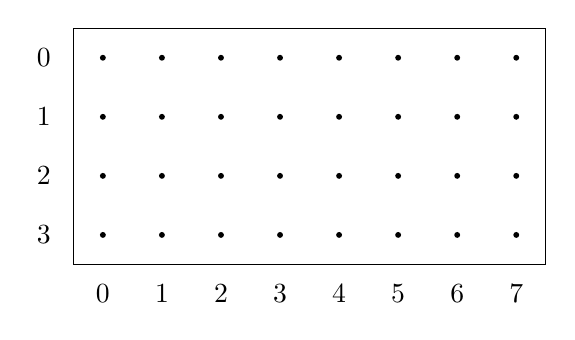
\begin{tikzpicture}[scale=0.75]
    \foreach \x in {0,...,7}
    \foreach \y in {0,...,3}
    {
      \fill (\x,\y) circle [radius=0.5mm,fill=black,draw] {};
    }
    \foreach \x in {0,...,7} \draw (\x, -1) node {\x};
    \foreach \y in {0,...,3} \draw (-1, 3 - \y) node {\y};
    \draw (-0.5,-0.5) -- (7.5,-0.5) -- (7.5,3.5) -- (-0.5,3.5) -- cycle;
  \end{tikzpicture}
\end{center}
As shown, both columns and rows are numbered consecutively, starting at 0.
The spacing between the sampling points must be uniform in both horizontal and vertical directions, and an anti-aliasing filter must be employed to limit the bandwidth of the image to satisfy the Nyquist-Shannon sampling theorem.

Each picture element detects the intensity of light transmitted or reflected at a sampling point in that particular position of the image, represented as one of 256 intensity levels, from 0 (minimum intensity) to 255 (maximum intensity).
Values between 0 and 255 represent intermediate intensities between these extremes.

\comment{I'm not sure how much of this should be explained in this document or elsewhere.}

In order to implement the image input device, you will need to add two extra cases to step \ref{itm:main-case} of the main procedure.

\begin{stepnumbers}[start=3]
\item If $k$ is
  \begin{description}
  \item[\READFRAME{}] then
    \begin{stepnumbers}
    \item Initialize the temporary 64-bit elements $c$ and $r$ to 0.
    \item Ready the next image to be consumed by the machine, and measure the intensity of light at all sampling points.
    \item Set $c$ to the number of columns in the image.
    \item \proc{Push} $c$.
    \item Set $r$ to the number of rows in the image.
    \item \proc{Push} $r$.
    \end{stepnumbers}
  \item[\READPIXEL{}] then
    \begin{stepnumbers}
    \item Initialize the temporary 64-bit elements $x$ and $y$ to 0.
    \item \proc{Pop} $x$.
    \item \proc{Pop} $y$.
    \item Find the intensity of light in the image at column $x$ and row $y$, represented as an 8-bit value, $z$.
    \item Push $z$.
    \end{stepnumbers}
  \end{description}
\end{stepnumbers}

\subsection{Image Output}

The \emph{Image Output} device allows the machine to produce an image represented as a two-dimensional array of points of color space values.
Moving images can be produced as a sequence of images.

\comment{Color space needs to be explained somewhere.}

In order to implement the image output device, you will need to add two extra cases to step \ref{itm:main-case} of the main procedure.

\begin{stepnumbers}[start=3]
\item If $k$ is
  \begin{description}
  \item[\NEWFRAME{}] then
    \begin{stepnumbers}
    \item Finish and render the frame constructed so far.
    \item Initialize the temporary 64-bit elements $r$, $w$, and $h$ to 0.
    \item \proc{Pop} $r$.
    \item \proc{Pop} $h$.
    \item \proc{Pop} $w$.
    \item Set the frame rate to $r$, the width of the frame to $w$, and the height of the frame to $h$.
    \end{stepnumbers}
  \item[\SETPIXEL{}] then
    \begin{stepnumbers}
    \item Initialize the temporary 64-bit elements  $x$, $y$, $r$, $g$, and $b$, to 0.
    \item \proc{Pop} $b$.
    \item \proc{Pop} $g$.
    \item \proc{Pop} $r$.
    \item \proc{Pop} $y$.
    \item \proc{Pop} $x$.
    \item Set the picture element at column $x$ and row $y$ to the point in the color space represented by the tuple $(r,g,b)$.
    \end{stepnumbers}
  \end{description}
\end{stepnumbers}

\subsection{Audio Output}

The \emph{Audio Output} device allows the machine to produce two-channel audio signal encoded digitally as Linear Pulse Code Modulation.
The device must create an audio signal in the form of a curve passing through a series of magnitude values.
Each channel value is in the range $\range{0}{2^{16}-1}$.

In order to implement the audio output device, you will need to add one extra case to step \ref{itm:main-case} of the main procedure.

\begin{stepnumbers}[start=3]
\item If $k$ is
  \begin{description}
  \item[\NEWFRAME{}] then
    \begin{stepnumbers}
    \item Initialize the temporary 64-bit elements  $l$ and $r$ to 0.
    \item \proc{Pop} $r$.
    \item \proc{Pop} $l$.
    \item Set the audio signal magnitude of the left channel to $l$.
    \item Set the audio signal magnitude of the right channel to $r$.
    \end{stepnumbers}
  \end{description}
\end{stepnumbers}

\subsection{Text Output}

In order to implement the text output device, you will need to add one extra case to step \ref{itm:main-case} of the main procedure.

\begin{stepnumbers}[start=3]
  \setcounter{enumi}{2}
\item If $k$ is
  \begin{description}
  \item[\PUTCHAR{}] then
    \begin{stepnumbers}
    \item Initialize the temporary 64-bit element $c$ to 0.
    \item \proc{Pop} $c$.
    \item Produce the character with Unicode code point $c$.
    \end{stepnumbers}
  \end{description}
\end{stepnumbers}

\section{Installing the Initial Program}

You first need to obtain the intial program from elsewhere on the film as a sequence of octets in hexadecimal notation.
These octets must be stored consecutively in $\MEM{}$, from index $0$ and up.

\comment{Describe how to supply parameters.}

When this is done, the machine can now be started, and it can then load a program from the film and execute it.

\appendix


\section{Number Notation}
\label{sec:number-notation}

\subsection{Binary Notation}
\label{sec:binary-notation}

Each element contains a value represented as a sequence of binary digits.
In this documentation, individual binary digits are referred to using non-negative integers, listed in decreasing order.
For an $n$-bit value, the individual bits, $b_i$, are numbered as follows:
\[ b_{n-1} \; b_{n-2} \; \ldots \; b_{1} \; b_{0} \]
When an $n$-bit binary element is interpreted as a non-negative integer, the value of that integer is
\[
    v = \sum_{i=0}^{n-1} b_{i}2^{i}
\]

\subsection{Hexadecimal Notation}
\label{sec:hexadecimal-notation}

For convenience, binary numbers are normally written in hexadecimal notation.
Each hexadecimal digit corresponds to a group of four binary digits, as shown in the following table.

\begin{center}
  \begin{tabular}{@{}ll@{}}
    \hline
    Hexadecimal digit & Binary digits \\
    \hline
    \num{0}           & \num{0000}   \\
    \num{1}           & \num{0001}   \\
    \num{2}           & \num{0010}   \\
    \num{3}           & \num{0011}   \\
    \num{4}           & \num{0100}   \\
    \num{5}           & \num{0101}   \\
    \num{6}           & \num{0110}   \\
    \num{7}           & \num{0111}   \\
    \hline
  \end{tabular}
  \hfil
  \begin{tabular}{@{}ll@{}}
    \hline
    Hexadecimal digit & Binary digits \\
    \hline
    \num{8}           & \num{1000}   \\
    \num{9}           & \num{1001}   \\
    \num{A}           & \num{1010}   \\
    \num{B}           & \num{1011}   \\
    \num{C}           & \num{1100}   \\
    \num{D}           & \num{1101}   \\
    \num{E}           & \num{1110}   \\
    \num{F}           & \num{1111}   \\
    \hline
  \end{tabular}
\end{center}

\end{document}
